\chapter{Тестирование}
Тестирование результатов выполнялось в два этапа: тестирование для найденных филогенетических паттернов и тестирование
восстановления деревьев с помощью MGRA2.

\section{Тестирование найденных паттернов}
В тестировании на симуляционных данных используется консервативная проверка правильности восстановления -
если восстановленное дерево не совпадает с верным (RF-метрика~\cite{Robinson1981} не дает расстояние 0)
или, в случае тестирования паттернов, другое дерево из возможных имеет ту же оценку, то дерево считается неправильно восстановленным.

\subsection{Тестирование на геномах со случайными брейкпоинт-графами}
Для тестирования найденных паттернов использовался подход описанный Wei Xu~\cite{xu2010exploring}.
Генерировались случайные геномы, состоящие из одной циклической хромосомы с 200 генами.
\begin{figure}[H]
  \centering
  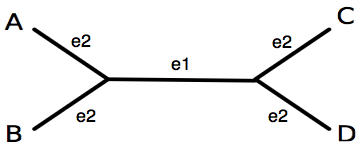
\includegraphics[max width=0.7\textwidth]{fig/3/wei_xu_tree.png}
  \caption{Филогенетическое дерево симулированных геномов~\cite{xu2010exploring}}
  \label{fig:testing_phyl_tree}
\end{figure}
\vspace{-1em}На~\ref{fig:testing_phyl_tree} показано филогенетическое дерево по которому генерировались тестовые четверки геномов.
Для генерации использовались значения $e_1 = v5, e_2 = v1 = v2 = v3 = v4$,
$e_1 = 1..5$, $e_2 = 5, 10, 20, 30, 40, 50, 60$.
Для каждой пары значений $(e_1, e_2)$ генерировалось 1000 четверок геномов с случайно выбранной топологией.
Результаты тестирования (доли правильно восстановленных деревьев для разных оценок)
приведены в таблице ниже. Оценки $S_{CA}$ и $S_{MCA}$ взяты из~\cite{xu2010exploring},
оценка $S_{MCA+}$ получается включением информации полученной из филогенетических паттернов в оценку $S_{MCA}$.
\begin{table}[H]
  \centering
  \begin{tabular}{|l|l|l|l|l|lllll}
    \hline
    e1 & e2 & CA    & MCA   & MCA+  & \multicolumn{1}{l|}{e1} & \multicolumn{1}{l|}{e2} & \multicolumn{1}{l|}{CA}    & \multicolumn{1}{l|}{MCA}   & \multicolumn{1}{l|}{MCA+}  \\ \hline
    1  & 5  & 0.768 & 0.92  & 0.925 & \multicolumn{1}{l|}{4}  & \multicolumn{1}{l|}{5}  & \multicolumn{1}{l|}{1.0}   & \multicolumn{1}{l|}{1.0}   & \multicolumn{1}{l|}{1.0}   \\ \hline
    1  & 10 & 0.572 & 0.721 & 0.728 & \multicolumn{1}{l|}{4}  & \multicolumn{1}{l|}{10} & \multicolumn{1}{l|}{0.993} & \multicolumn{1}{l|}{0.999} & \multicolumn{1}{l|}{0.999} \\ \hline
    1  & 20 & 0.434 & 0.515 & 0.518 & \multicolumn{1}{l|}{4}  & \multicolumn{1}{l|}{20} & \multicolumn{1}{l|}{0.877} & \multicolumn{1}{l|}{0.959} & \multicolumn{1}{l|}{0.96}  \\ \hline
    1  & 30 & 0.39  & 0.432 & 0.44  & \multicolumn{1}{l|}{4}  & \multicolumn{1}{l|}{30} & \multicolumn{1}{l|}{0.749} & \multicolumn{1}{l|}{0.832} & \multicolumn{1}{l|}{0.836} \\ \hline
    1  & 40 & 0.39  & 0.421 & 0.426 & \multicolumn{1}{l|}{4}  & \multicolumn{1}{l|}{40} & \multicolumn{1}{l|}{0.659} & \multicolumn{1}{l|}{0.734} & \multicolumn{1}{l|}{0.738} \\ \hline
    1  & 50 & 0.384 & 0.407 & 0.413 & \multicolumn{1}{l|}{4}  & \multicolumn{1}{l|}{50} & \multicolumn{1}{l|}{0.599} & \multicolumn{1}{l|}{0.656} & \multicolumn{1}{l|}{0.667} \\ \hline
    1  & 60 & 0.346 & 0.36  & 0.368 & \multicolumn{1}{l|}{4}  & \multicolumn{1}{l|}{60} & \multicolumn{1}{l|}{0.516} & \multicolumn{1}{l|}{0.559} & \multicolumn{1}{l|}{0.572} \\ \hline
    2  & 5  & 0.984 & 1.0   & 1.0   & \multicolumn{1}{l|}{5}  & \multicolumn{1}{l|}{5}  & \multicolumn{1}{l|}{1.0}   & \multicolumn{1}{l|}{1.0}   & \multicolumn{1}{l|}{1.0}   \\ \hline
    2  & 10 & 0.849 & 0.944 & 0.944 & \multicolumn{1}{l|}{5}  & \multicolumn{1}{l|}{10} & \multicolumn{1}{l|}{0.999} & \multicolumn{1}{l|}{1.0}   & \multicolumn{1}{l|}{1.0}   \\ \hline
    2  & 20 & 0.624 & 0.756 & 0.758 & \multicolumn{1}{l|}{5}  & \multicolumn{1}{l|}{20} & \multicolumn{1}{l|}{0.957} & \multicolumn{1}{l|}{0.988} & \multicolumn{1}{l|}{0.989} \\ \hline
    2  & 30 & 0.542 & 0.611 & 0.619 & \multicolumn{1}{l|}{5}  & \multicolumn{1}{l|}{30} & \multicolumn{1}{l|}{0.847} & \multicolumn{1}{l|}{0.927} & \multicolumn{1}{l|}{0.927} \\ \hline
    2  & 40 & 0.486 & 0.55  & 0.562 & \multicolumn{1}{l|}{5}  & \multicolumn{1}{l|}{40} & \multicolumn{1}{l|}{0.721} & \multicolumn{1}{l|}{0.792} & \multicolumn{1}{l|}{0.798} \\ \hline
    2  & 50 & 0.446 & 0.48  & 0.488 & \multicolumn{1}{l|}{5}  & \multicolumn{1}{l|}{50} & \multicolumn{1}{l|}{0.657} & \multicolumn{1}{l|}{0.709} & \multicolumn{1}{l|}{0.714} \\ \hline
    2  & 60 & 0.413 & 0.439 & 0.449 & \multicolumn{1}{l|}{5}  & \multicolumn{1}{l|}{60} & \multicolumn{1}{l|}{0.601} & \multicolumn{1}{l|}{0.651} & \multicolumn{1}{l|}{0.656} \\ \hline
    3  & 5  & 1.0   & 1.0   & 1.0   &                         &                         &                            &                            &                            \\ \cline{1-5}
    3  & 10 & 0.963 & 0.997 & 0.997 &                         &                         &                            &                            &                            \\ \cline{1-5}
    3  & 20 & 0.777 & 0.874 & 0.878 &                         &                         &                            &                            &                            \\ \cline{1-5}
    3  & 30 & 0.659 & 0.754 & 0.758 &                         &                         &                            &                            &                            \\ \cline{1-5}
    3  & 40 & 0.625 & 0.688 & 0.693 &                         &                         &                            &                            &                            \\ \cline{1-5}
    3  & 50 & 0.526 & 0.585 & 0.601 &                         &                         &                            &                            &                            \\ \cline{1-5}
    3  & 60 & 0.481 & 0.528 & 0.542 &                         &                         &                            &                            &                            \\ \cline{1-5}
  \end{tabular}
  \caption{Результаты тестирования на геномах со случайными брейкпоинт-графами}
  \label{table:second_group}
\end{table}

Как видно из таблицы~\ref{table:second_group}, использование информации,
получаемой с помощью филогенетических паттернов дает улучшение эффективности восстановления относительно оценки $S_{MCA}$ от 0 до 1.5\%.
На основе того, что в некоторых случаях улучшений от использования информации полученной из филогенетических паттернов не происходило,
было выдвинуто предположение, что паттернов в брейкпоинт-графе в данных случаях не встречалось и
проведено тестирование на случайных геномах, в брейкпоинт-графах которых гарантированно были искомые паттерны.

\subsection{Тестирование на геномах с отфильтрованными брейкпоинт-графами}
Генерация геномов производилась тем же образом, что и в предыдущем случае, но на параметрах $e_1 = 4, e_2 = 60$.
Было сгенерировано 20434 четверки геномов, из которых 1001 четверка содержала паттерны \q{мешок} и \q{цилиндр},
и 10001 хотя бы паттерн \q{мешок}.
\begin{table}[H]
\caption{Тестирование на геномах с отфильтрованными брейкпоинт-графами}
\label{table:filtered_graphs}
\begin{tabular}{|l|l|l|l|l|}
\hline
Паттерн                     & Доля  & CA     & MCA    & MCA+  \\ \hline
\q{мешок}                   & 0.489 & 0.5386 & 0.5848 & 0.602 \\ \hline
\q{мешок} и \q{цилиндр}     & 0.049 & 0.586  & 0.619  & 0.644 \\ \hline
\end{tabular}
\end{table}

Результаты представлены в таблице~\ref{table:filtered_graphs}, столбец \q{Доля} обозначает долю брейкпоинт-графов с указанной конфигурацией
от общего числа сгенерированных. Почти в половине случаев брейкпоинт-граф случайно сгенерированной четверки геномов содержал
хотя бы паттерн \q{мешок} и в этом случае наблюдалось улучшение эффективности восстановления относительно оценки $S_{MCA}$ на 1.72\%.
В случае присутствия и паттерна \q{мешок} и паттерна \q{цилиндр} (а это наблюдалось в примерно 5\% случаев) улучшение составило 2.5\%.

\section{Тестирование восстановления с помощью MGRA2}
\subsection{Тестирование на симуляционных данных}
Для тестирования восстановления деревьев с помощью MGRA2 генерировались случайные деревья на $N = 6, 10, 12$ геномах.
Каждый геном состоял из $G = 1000, 1500$ блоков.
На наборе из $N$ геномов строилось случайное полное бинарное дерево с $N$ листьями, далее проводился симуляционный процесс вдоль каждой ветки:
при прохождении по ветке геном претерпевал случайное число эволюционных событий из диапазона $\lbrack \frac{E}{2}, E \rbrack$,
где $E = 100, 200$; $ID = 0.2, 0.4, 0.6$ из этих событий были вставками или удалениями одного блока, вставки и удаления происходили равновероятно.
Для сравнения в тестировании были взяты инструменты TIBA, GAS Phylogeny, MLWD и выделен компонент TreeInferer из инструмента Ragout.
MGRA2 запускался на двух оценках - \q{распределение} и \q{простые пути}.
Первая оценка использует как \q{свидетельства} ребра: если $\bb{Q}$ - все множество цветов,
то каждое ребро цвета $Q$ добавляет 1 к оценке разделения $Q|\bb{Q} \setminus Q$.
Вторая оценка использует идею простых путей и циклов в брейкпоинт-графе - путей и циклов, состоящих из вершин мультистепени 2,
также ищет паттерны \q{мешок} и \q{цилиндр} (присутствующие в них двойные ребра используются как свидельства того, что геномы
их составляющие должны быть вместе).
где ребра имеют цвета попеременно $Q$ и $\bb{Q} \setminus Q$.
Тестирование разделено на 2 части - с вставками и удалениями и без них.
В первой части участвуют все инструменты, во второй - только MGRA2 и MLWD,
так как другие не могут работать с данными в которых были вставки и удаления.

\subsubsection{Тестирование без вставок и удалений}
\begin{table}[H]
\caption{Результы тестирования на симуляционных данных без вставок и удалений}
\label{table:no_indel_results}
\begin{tabular}{|l|l|l|l|l|l|l|l|l|}
\hline
\multicolumn{1}{|c|}{G} & \multicolumn{1}{c|}{N} & \multicolumn{1}{c|}{E} & \multicolumn{1}{c|}{GAS P} & \multicolumn{1}{c|}{TIBA} & \multicolumn{1}{c|}{TreeInferer} & \multicolumn{1}{c|}{MLWD} & \multicolumn{1}{c|}{MGRA2\_D} & \multicolumn{1}{c|}{MGRA2\_SP} \\ \hline
1000                    & 6                      & 100                    & 1.0                        & 1.0                       & 1.0                             & 1.0                       & 1.0                           & 1.0                            \\ \hline
1000                    & 6                      & 200                    & 1.0                        & 1.0                       & 1.0                             & 1.0                       & 1.0                           & 1.0                            \\ \hline
1000                    & 10                     & 100                    & 1.0                        & 1.0                       & 1.0                             & 1.0                       & 1.0                           & 1.0                            \\ \hline
1000                    & 10                     & 200                    & 1.0                        & 1.0                       & 1.0                             & 1.0                       & 0.8                           & 0.0                            \\ \hline
1000                    & 12                     & 100                    & 1.0                        & 1.0                       & 1.0                             & 1.0                       & 1.0                           & 0.5                            \\ \hline
1000                    & 12                     & 200                    & 1.0                        & 1.0                       & 0.9                             & 1.0                       & 0.7                           & 0.0                            \\ \hline
1500                    & 6                      & 100                    & 1.0                        & 1.0                       & 1.0                             & 1.0                       & 1.0                           & 1.0                            \\ \hline
1500                    & 6                      & 200                    & 1.0                        & 1.0                       & 1.0                             & 1.0                       & 1.0                           & 1.0                            \\ \hline
1500                    & 10                     & 100                    & 1.0                        & 1.0                       & 1.0                             & 1.0                       & 1.0                           & 1.0                            \\ \hline
1500                    & 10                     & 200                    & 1.0                        & 1.0                       & 1.0                             & 1.0                       & 1.0                           & 0.9                            \\ \hline
1500                    & 12                     & 100                    & 1.0                        & 1.0                       & 1.0                             & 1.0                       & 1.0                           & 1.0                            \\ \hline
1500                    & 12                     & 200                    & 1.0                        & 1.0                       & 1.0                             & 1.0                       & 1.0                           & 0.5                            \\ \hline
\end{tabular}
\end{table}

Как видно из таблицы~\ref{table:no_indel_results}, вторая оценка, обозначенная как MGRA2\_SP не показала ожидаемой эффективности
(учитывая то, что она использует обобщенный паттерн, введенный Wei Xu),
когда первая оценка, обозначенная как MGRA2\_D, либо сравнивалась, либо незначительно проигрывала в эффективности восстановления существующим инструментам.

\subsubsection{Тестирование со вставками и удалениями}
\begin{table}[H]
\centering
\begin{tabular}{|l|l|l|l|l|l|l|l|l|l|l|l|l|l|}
\hline
\multicolumn{1}{|c|}{G} & \multicolumn{1}{c|}{N} & \multicolumn{1}{c|}{E} & \multicolumn{1}{c|}{ID} & \multicolumn{1}{c|}{MLWD} & \multicolumn{1}{c|}{D} & \multicolumn{1}{c|}{SP} & \multicolumn{1}{c|}{G} & \multicolumn{1}{c|}{N} & \multicolumn{1}{c|}{E} & \multicolumn{1}{c|}{ID} & \multicolumn{1}{c|}{MLWD} & \multicolumn{1}{c|}{D} & \multicolumn{1}{c|}{SP} \\ \hline
1000                    & 6                      & 100                    & 20                      & 1.0                       & 1.0                    & 1.0                     & 1500                   & 6                      & 100                    & 20                      & 1.0                       & 1.0                    & 1.0                     \\ \hline
1000                    & 6                      & 100                    & 40                      & 1.0                       & 1.0                    & 1.0                     & 1500                   & 6                      & 100                    & 40                      & 1.0                       & 1.0                    & 1.0                     \\ \hline
1000                    & 6                      & 100                    & 60                      & 1.0                       & 1.0                    & 1.0                     & 1500                   & 6                      & 100                    & 60                      & 1.0                       & 1.0                    & 1.0                     \\ \hline
1000                    & 6                      & 200                    & 20                      & 1.0                       & 1.0                    & 1.0                     & 1500                   & 6                      & 200                    & 20                      & 1.0                       & 1.0                    & 1.0                     \\ \hline
1000                    & 6                      & 200                    & 40                      & 1.0                       & 1.0                    & 1.0                     & 1500                   & 6                      & 200                    & 40                      & 1.0                       & 1.0                    & 1.0                     \\ \hline
1000                    & 6                      & 200                    & 60                      & 1.0                       & 1.0                    & 1.0                     & 1500                   & 6                      & 200                    & 60                      & 1.0                       & 1.0                    & 1.0                     \\ \hline
1000                    & 10                     & 100                    & 20                      & 1.0                       & 1.0                    & 1.0                     & 1500                   & 10                     & 100                    & 20                      & 1.0                       & 1.0                    & 1.0                     \\ \hline
1000                    & 10                     & 100                    & 40                      & 1.0                       & 1.0                    & 1.0                     & 1500                   & 10                     & 100                    & 40                      & 1.0                       & 1.0                    & 1.0                     \\ \hline
1000                    & 10                     & 100                    & 60                      & 1.0                       & 1.0                    & 1.0                     & 1500                   & 10                     & 100                    & 60                      & 1.0                       & 1.0                    & 1.0                     \\ \hline
1000                    & 10                     & 200                    & 20                      & 1.0                       & 1.0                    & 0.4                     & 1500                   & 10                     & 200                    & 20                      & 1.0                       & 1.0                    & 1.0                     \\ \hline
1000                    & 10                     & 200                    & 40                      & 1.0                       & 1.0                    & 0.9                     & 1500                   & 10                     & 200                    & 40                      & 1.0                       & 1.0                    & 1.0                     \\ \hline
1000                    & 10                     & 200                    & 60                      & 1.0                       & 1.0                    & 0.9                     & 1500                   & 10                     & 200                    & 60                      & 1.0                       & 1.0                    & 1.0                     \\ \hline
1000                    & 12                     & 100                    & 20                      & 1.0                       & 1.0                    & 1.0                     & 1500                   & 12                     & 100                    & 20                      & 1.0                       & 1.0                    & 1.0                     \\ \hline
1000                    & 12                     & 100                    & 40                      & 1.0                       & 1.0                    & 1.0                     & 1500                   & 12                     & 100                    & 40                      & 1.0                       & 1.0                    & 1.0                     \\ \hline
1000                    & 12                     & 100                    & 60                      & 1.0                       & 1.0                    & 1.0                     & 1500                   & 12                     & 100                    & 60                      & 1.0                       & 1.0                    & 1.0                     \\ \hline
1000                    & 12                     & 200                    & 20                      & 1.0                       & 0.6                    & 0.0                     & 1500                   & 12                     & 200                    & 20                      & 1.0                       & 1.0                    & 0.7                     \\ \hline
1000                    & 12                     & 200                    & 40                      & 1.0                       & 0.9                    & 0.2                     & 1500                   & 12                     & 200                    & 40                      & 1.0                       & 1.0                    & 0.8                     \\ \hline
1000                    & 12                     & 200                    & 60                      & 1.0                       & 1.0                    & 0.4                     & 1500                   & 12                     & 200                    & 60                      & 1.0                       & 1.0                    & 1.0                     \\ \hline
\end{tabular}
\caption{Результы тестирования на симуляционных данных со вставками и удалениями}
\label{table:with_indel_results}
\end{table}

Как видно из таблицы~\ref{table:with_indel_results}, вторая оценка, обозначенная как SP, опять показала меньшую
по сравнению с первой оценкой, обозначенной как D, эффективность, которая в этом тесте лишь в двух случаях не восстановила все деревья идеально.

\subsection{Тестирование на реальных данных}
Для тестирования на реальных данных использовались данные предоставленные московской лабораторией М. С. Гельфанда.
Для тестирования использовались два набора данных: из рода Burkholderia и рода Yersinia.

В первом случае было восстановленное MGRA2 дерево не совпало с полученным биологическими методами.
Далее было замечено, что количество перестроек для полученной биологически и восстановленной топологий отличается на 1 из 95,
после этого в лаборатории было построено дерево на основе матрицы наличия/отсутствия гена.
Это дерево совпало с восстановленным MGRA2.

Восстановленное MGRA2 из второго набора данных дерево совпало с полученным биологическими методами в делении на три основные пандемии чумы.
Несовпадения произошли в поддеревьях с сомнительной топологией полученного биологически дерева.
